\documentclass[a4paper,12pt]{article} % тип документа

% report, book

% Рисунки
\usepackage{graphicx}
\usepackage{wrapfig}
\usepackage{mathtext}
\usepackage[left=2cm,right=2cm,
    top=2cm,bottom=2cm,bindingoffset=0cm]{geometry}

\usepackage{hyperref}
\usepackage[rgb]{xcolor}
\hypersetup{				% Гиперссылки
    colorlinks=true,       	% false: ссылки в рамках
	urlcolor=blue          % на URL
}

%  Русский язык
\usepackage[T2A]{fontenc}			% кодировка
\usepackage[utf8]{inputenc}			% кодировка исходного текста
\usepackage[english,russian]{babel}	% локализация и переносы


% Математика
\usepackage{amsmath,amsfonts,amssymb,amsthm,mathtools} 
\usepackage{titlesec}
\titlelabel{\thetitle.\quad}

\usepackage{wasysym}

\author{Анна Назарчук Б02-109}
\title{3.5.1 Изучение плазмы газового разряда в неоне}
\date{}
\begin{document}
\maketitle
\section{Аннотация}
В работе изучается плазма газового разряда в неоне с помощью двойного зонда. Снимается ВАХ разряда в режиме поднормального тлеющего разряда. Получаются зондовые характеристики, рассчитываются параметры плазмы (например, $\omega_p$, $r_D$).


\section{Введение}
Как известно, вещество может находиться в трёх агрегатных состояниях
— твёрдом, жидком и газообразном, причём эти состояния последовательно
сменяются по мере возрастания температуры. Если и дальше
нагревать газ, то сначала молекулы диссоциируют на атомы, а затем и
атомы распадаются на электроны и ионы, так что газ становится ионизованным,
представляя собой смесь из свободных электронов и ионов,
а также нейтральных частиц. Если степень ионизации газа (отношение
числа ионизованных атомов к их полному числу) оказывается достаточно
велика, то поведение заряженных частиц приобретает коллективный характер,
так что описание свойств среды не может быть сведено к описанию
обычного газа, содержащего некоторое количество отдельных заряженных
частиц. Такое состояние ионизованного газа и называется плазмой. Первое описание плазмы было дано в 1923 г. И. Ленгмюром. Современная физика термин "газовый разряд" трактует как не только процесс протекания тока через газ, но и любой процесс возникновения ионизации газа под действием внешнего поля. Это и планируется пронаблюдать в данной работе.

\section{Поставка задачи}
Получить вольт-амперную характеристику газового разряда, определить тип разряда. Рассчитать основные характеристики плазмы методом зондовых характеристик.


\section{Теоретические сведения}
Определяющими свойствами плазмы являются коллективный характер
её движения и квазинейтральность (равенство нулю средней плотности
заряда). Рассмотрим простейший вид коллективных плазменных
колебаний.

\begin{equation}
\label{w_p}
\omega_p=\sqrt{\frac{4\pi n_e e^2}{m_e}}
\end{equation}
$\omega_p$ - плазменная частота (частота коллективных колебаний электронов относительно квазинейтрального состояния, так называемых ленгмюровских колебаний, определяет временной масштаб для плазмы)

Плазменный масштаб плазменных явлений задается дебаевским радиусом - амплитудой ленгмюровских колебаний, возбуждаемых тепловыми колебаниями
\begin{equation}
r_D = \sqrt{\frac{k_Б T_e}{4\pi n_e e^2}}
\end{equation}

Рассмотрим плазменное экранирование. В равновесную плазму ($T = T_e = T_i$) помещена массивная пробная частица заряда $+q$, с радиусом, большим $r_D$. Для электронов из закона Больцмана:
\begin{equation}
n_e = n_{e0}\cdot \exp(\frac{e\varphi}{k_Б T})
\end{equation} 

Аналогичное соотношение можно написать и для ионов (однозарядных). Температура электронов достаточно высока, поэтому:
\begin{equation}
\rho = -en_e+en_i\approx -en\cdot \frac{e\varphi}{k_Б T}
\end{equation}

Уравнение Пуассона для одномерного случая:
\begin{equation}
\frac{d^2 \varphi}{dx^2}=-4\pi \rho
\end{equation}

Объединив два уравнения, получим аналогичное выражение:
\begin{equation}
r_D = \sqrt{\frac{k_Б T_e}{4\pi n_e e^2}}
\end{equation}

Теперь рассмотрим неравновесную плазму ($T_e\neq T_i$):
\begin{equation}
\label{R_De}
r_{De} = \sqrt{\frac{k_Б T_e}{4\pi n_e e^2}}, \hspace{2mm} 
r_{Di} = \sqrt{\frac{k_Б T_i}{4\pi n_i e^2}}
\end{equation}

Поэтому в общем случае:
\begin{equation}
\label{r_D_общ}
r_D = (r_{De}^2+r_{Di}^2)^{-1/2} = \sqrt{\frac{k_Б}{4\pi n_e e^2}\frac{T_eT_i}{T_e+T_i}}=
\end{equation}

Плазма - ионизированный газ, $r_D \ll a$, размера области, занимаемой газом.
Плазма идеальна, если кулоновская энергия мала по сравнению с тепловой:
\begin{equation}
\omega_{кул} = -\frac{1}{2}n_i\frac{q^2}{r_D}, \hspace{2mm} \omega_{тепл} = n_ik_БT
\end{equation} 

Отношение энергий есть число заряженных частиц в сфере с дебаевским радиусом:
\begin{equation}
\label{N_D}
N_D = \frac{4}{3}\pi n_ir^3_D
\end{equation}

Плазма идеальна при $N_D\gg1$.

\section{Методика измерений}
\subsection{Плавающий потенциал}
Измерение электрических потенциалов с помощью "зондов" - небольших проводников, вводимых в плазму. При внесении проводника в плазму, он подвергается "бомбардировке" со стороны её заряженных частиц. Из-за различий в скорости частиц проводник зарядится отрицательно с потенциалов (отн. плазмы) $-U_f$ - плавающий потенциал.
Если бы $U_f = 0$:
\begin{equation}\label{i_0}
I_{e0} = \frac{n\bar{\upsilon_e}}{4}eS, \hspace{2mm} I_{i0} = \frac{n\bar{\upsilon_i}}{4}eS, 
\end{equation}

Теперь $U_f \neq 0$: $I_i \approx I_{i0}$, согласно распределению Больцмана:
\begin{equation}
I_e = I_{e0} \exp(\frac{eU_f}{k_БT_e})
\end{equation}

\subsection{Одиночный зонд}
Схема измерений приведена на рис. \ref{одиночный}. 
\begin{figure}[h!]
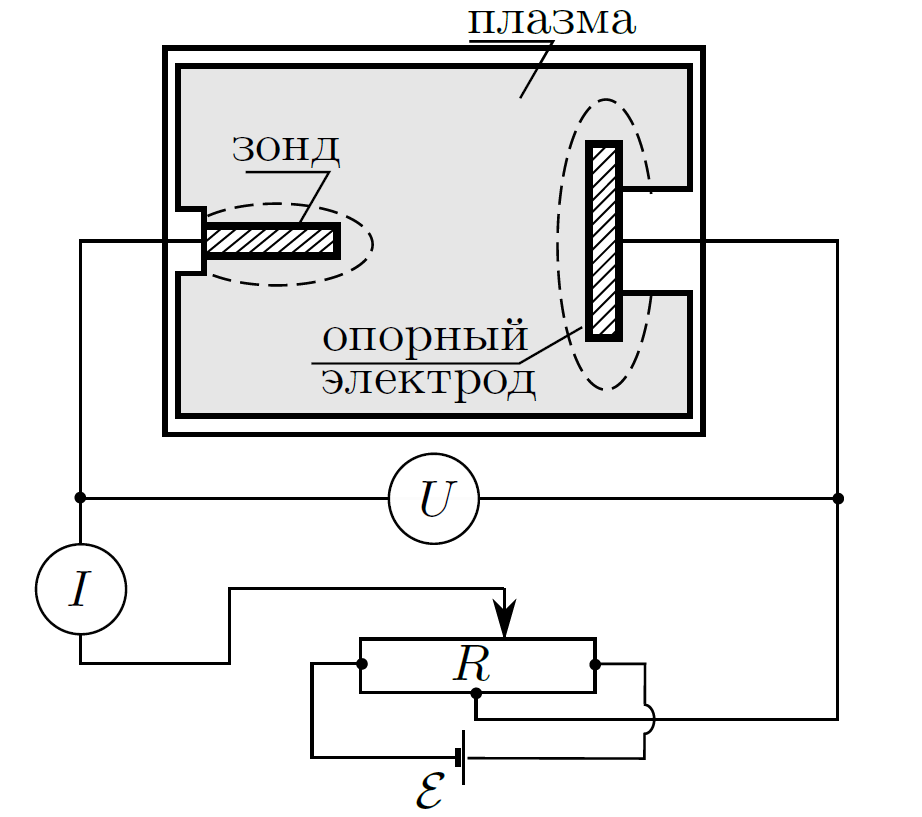
\includegraphics[width=0.3\textwidth]{Одиночный}
\caption{Исследование плазмы методом одиночного зонда} \label{одиночный}
\end{figure}

Зависимость тока через зонд от потенциала зонда - зондовая характеристика (рис. \ref{зондовая_характеристика}). 
\begin{figure}[h!]
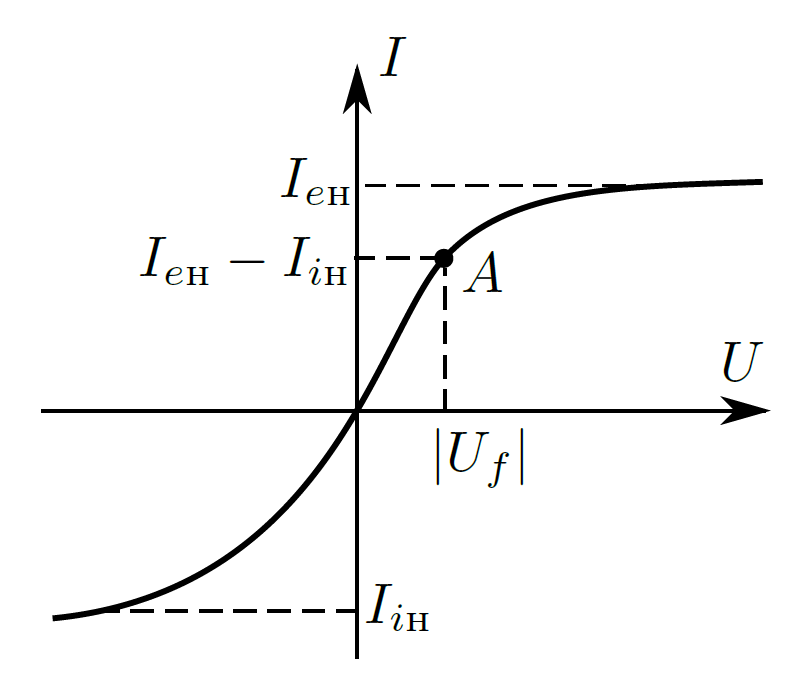
\includegraphics[width=0.3\textwidth]{Зондовая_характеристика}
\caption{Зондовая характеристика} \label{зондовая_характеристика}
\end{figure}
Токи можно оценить из формулы \ref{i_0}:
\begin{equation}
I_{ен} \approx I_{e0} = \frac{1}{4}n_eS\sqrt{\frac{8k_БT_e}{\pi m_e}}
\end{equation}
Полуэмпирическая формула Д. Бома:
\begin{equation} 
\label{бом}
I_{iн} \approx 0.4 n_iS\sqrt{\frac{2k_БT_e}{m_i}}
\end{equation}

\subsection{Двойной зонд}
Двойной зонд - система, состоящая из двух одинаковых зондов на небольшом растоянии друг от друга, между которыми создается небольшая (по сравнению с $U_f$) разность потенциалов $U$. При малых токах через зонд:
\begin{equation}
U_1 = U_f +\Delta U_1, \hspace{2mm} U_2 = U_f +\Delta U_2
\end{equation}
\begin{equation}
U = U_2 - U_1 = \Delta U_2 -\Delta U_1
\end{equation}
Токи, приходящие на электроды:
\begin{equation}
I_1 = I_{iн}(1-\exp(\frac{e\Delta U_1}{k_БT_e})), \hspace{2mm} 
I_2 = I_{iн}(1-\exp(\frac{e\Delta U_2}{k_БT_e}))
\end{equation}
Из последовательного соединения зондов:
\begin{equation}
I = I_{iн} th\frac{eU}{2k_БT_e}
\end{equation}
Вблизи $U = 0$:
\begin{equation}
\label{двойной_зонд}
k_БT_e = \frac{1}{2}\frac{eI_{iн}}{\frac{dI}{dU}|_{U=0}}
\end{equation}

\subsection{Установка}
Схема экспериментальной установки приведена на рисунке \ref{установка}. Трубка наполнена изотопом неона $^{22}Ne$ при давлении 2 мм рт. ст. При подключении к ВИП анода-I между ним и катодом возникает газовый разряд. Ток разряда измеряется миллиамперметром $A_1$, а падение
напряжения на разрядной трубке — вольтметром $V_1$. При подключении к ВИП анода-II разряд возникает в пространстве между катодом и анодом-II, где находится двойной зонд, используемый
для диагностики плазмы положительного столба.
\begin{figure}[h!]
\begin{center}
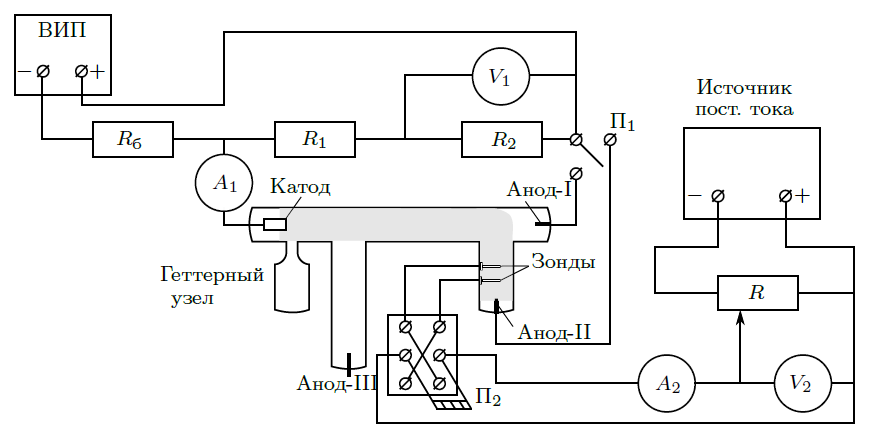
\includegraphics[width=0.6\textwidth]{Установка}
\caption{Схема установки} \label{установка}
\end{center}
\end{figure}

\section{Измерения и обработка данных}
\subsection{Вольт-амперная характеристика разряда}
С помощью вольтметра $V_1$ и амперметра $A_1$ измерили вольт-амперную
характеристику разряда $I_p(U_p)$ (рис. \ref{ВАХ_разряда})

\begin{figure}[h!]
\begin{center}
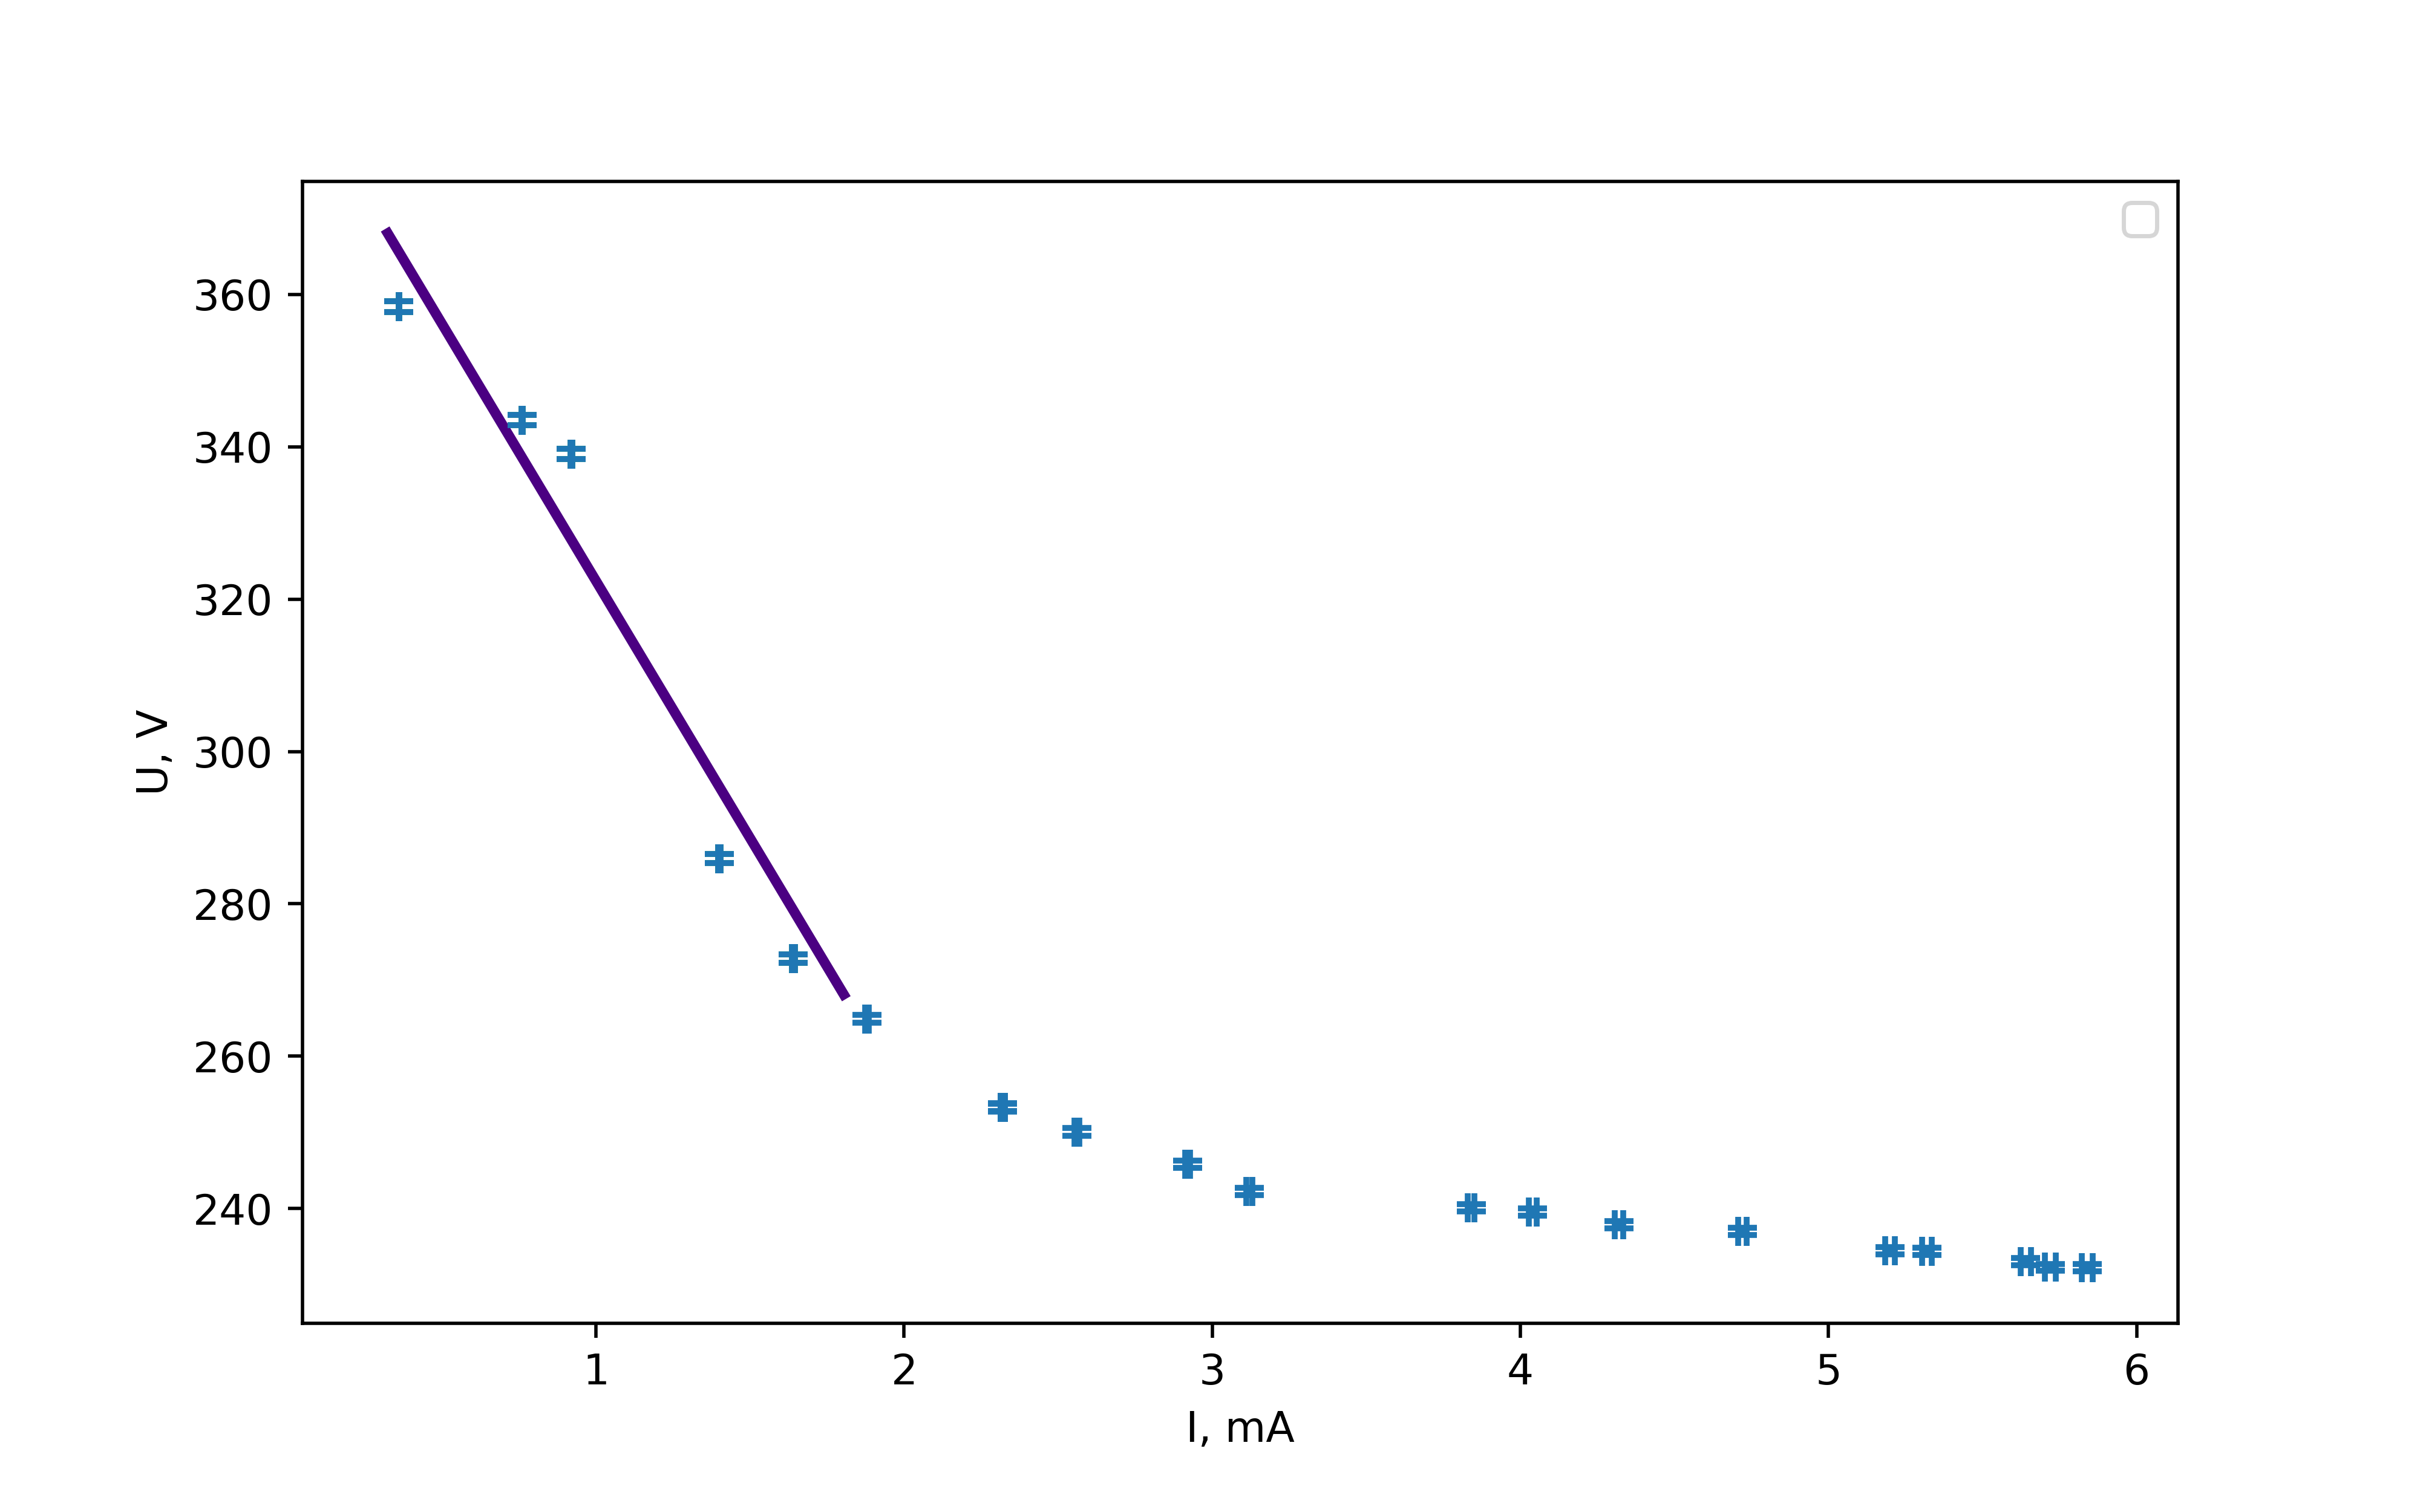
\includegraphics[width=\textwidth]{U(I)_discharge}
\caption{ВАХ разряда} \label{ВАХ_разряда}
\end{center}
\end{figure}

По наклону кривой определили максимальное $R_{диф}=\frac{dU}{dI} = -68000 \pm 11000$ Ом. Полученный участок ВАХ соответствует поднормальному тлеющему разряду.

\subsection{Зондовые характеристики} 
При фиксированном токе разряда измерили вольт-амперную характеристику двойного зонда. (рис. \ref{ВАХ_зонда}). Для каждой зондовой характеристики определили ионный ток и наклон характеристики в начале координат по графику. Из полученных результатов рассчитаны $T_e$ (ф-ла \ref{двойной_зонд}), $n_i$ (ф-ла \ref{бом}), $\omega_p$ (ф-ла \ref{w_p}), $r_{De}$ (ф-ла \ref{R_De}) , $r_D$(ф-ла \ref{r_D_общ}), $N_D$ (ф-ла \ref{N_D}), $\alpha$ - степень ионизации плазмы. Результаты приведены в таблице \ref{data}, также построены графики зависимости 
электронной температуры и концентрации электронов от тока разряда (рис. \ref{от_тока_разряда}).

\begin{figure}[h!]
\begin{center}
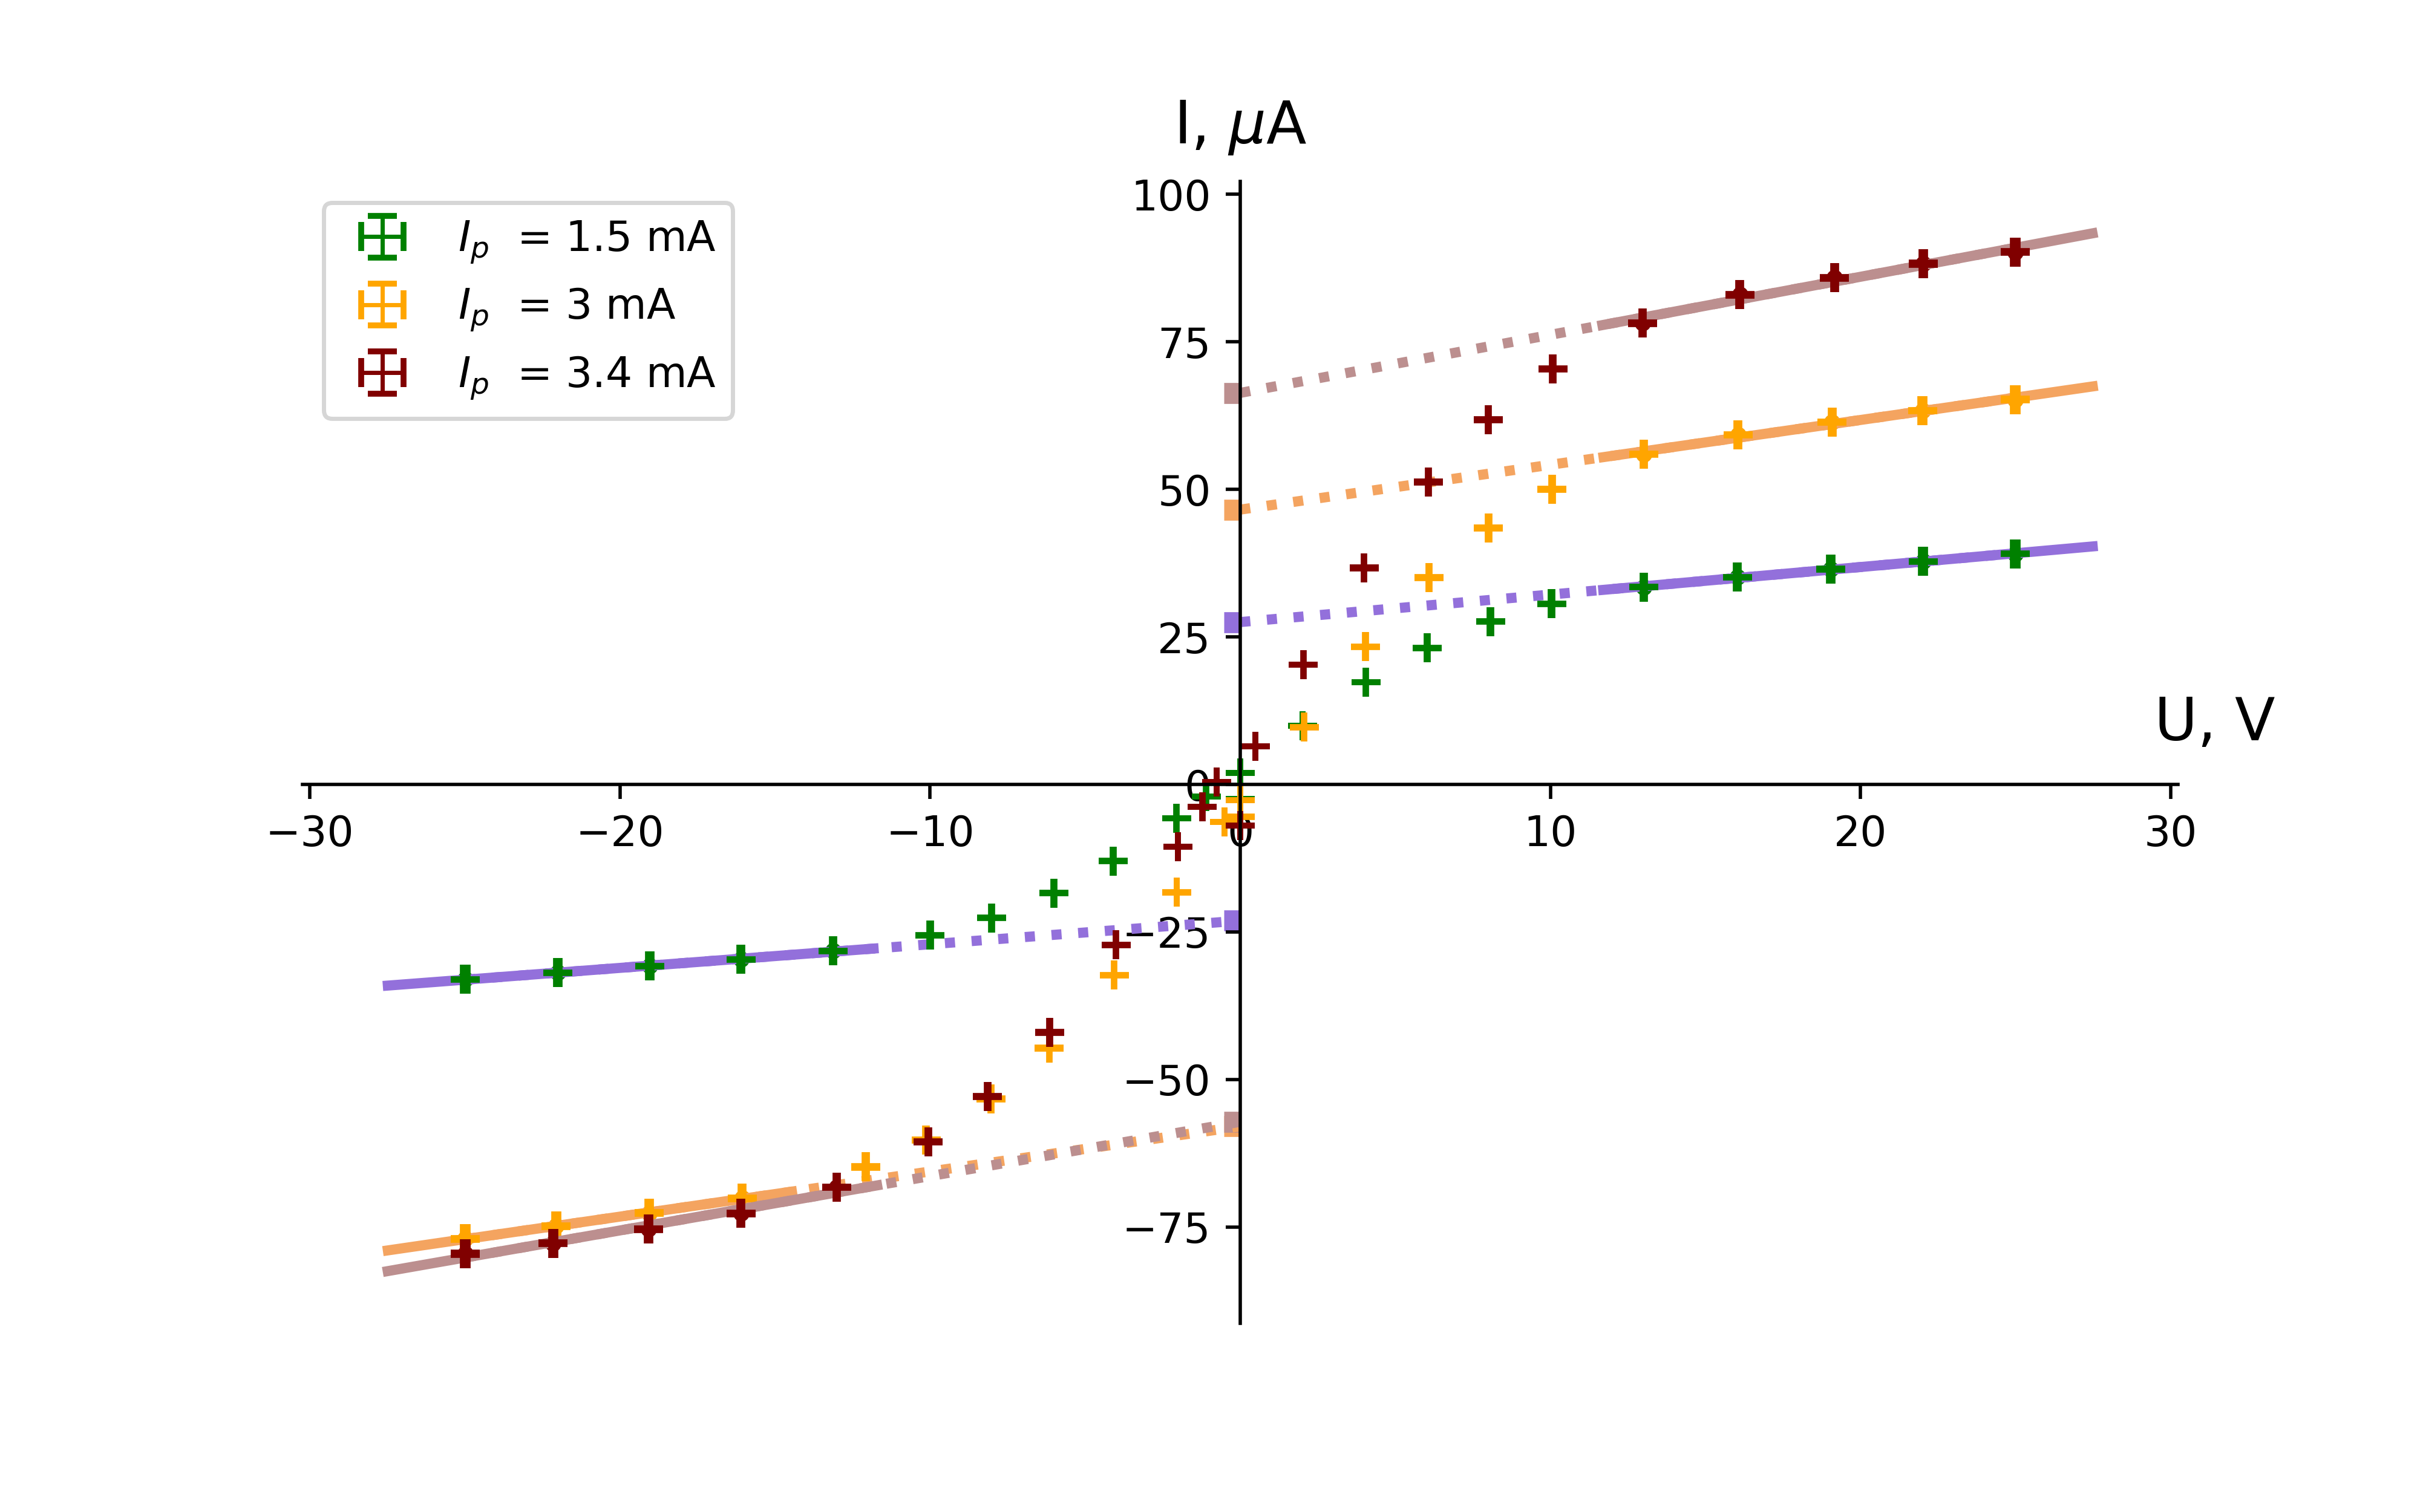
\includegraphics[width=\textwidth]{I(U)_probe}
\caption{ВАХ двойного зонда} \label{ВАХ_зонда}
\end{center}
\end{figure}

\begin{table}[h!]
\caption{Характеристики плазмы для разных токов разряда $I_p$}
\label{data}
\begin{tabular}{|l|l|l|l|}
\hline
$I_p,$ мА                & 1.5               & 3                 & 3.4               \\ \hline
$T_e,$ эВ                & $ 3.1 \pm 0.2 $   & $ 4.2 \pm 0.1 $   & $ 3.7 \pm 0.4 $   \\ \hline
$n_i, 10^{10}$ $ 1/см^3$    & $ 2.1 \pm 0.1 $   & $ 4.6 \pm 0.1 $   & $ 4.8 \pm 0.3 $   \\ \hline
$\omega_p, 10^{9}$ $ рад/с$ & $ 8.2 \pm 0.2 $   & $ 12.0 \pm 0.1 $  & $ 12.4 \pm 0.4 $  \\ \hline
$r_{De}, 10^{-3} $ $см$     & $ 9.0 \pm 0.8 $   & $ 7.2 \pm 0.2 $   & $ 6.5 \pm 0.7 $   \\ \hline
$r_{D}, 10^{-3} $ $см$      & $ 0.82 \pm 0.03 $ & $ 0.56 \pm 0.01 $ & $ 0.54 \pm 0.03 $ \\ \hline
$N_{D}$                  & $ 49 \pm 6 $      & $ 34 \pm 1 $      & $ 33 \pm 6 $      \\ \hline
$\alpha, 10^{-5}$        & $ 3.9 \pm 0.4 $   & $ 11.6 \pm 0.3 $  & $ 10.7 \pm 1.2 $  \\ \hline
\end{tabular}
\end{table}

\begin{figure}[h!]
\begin{center}
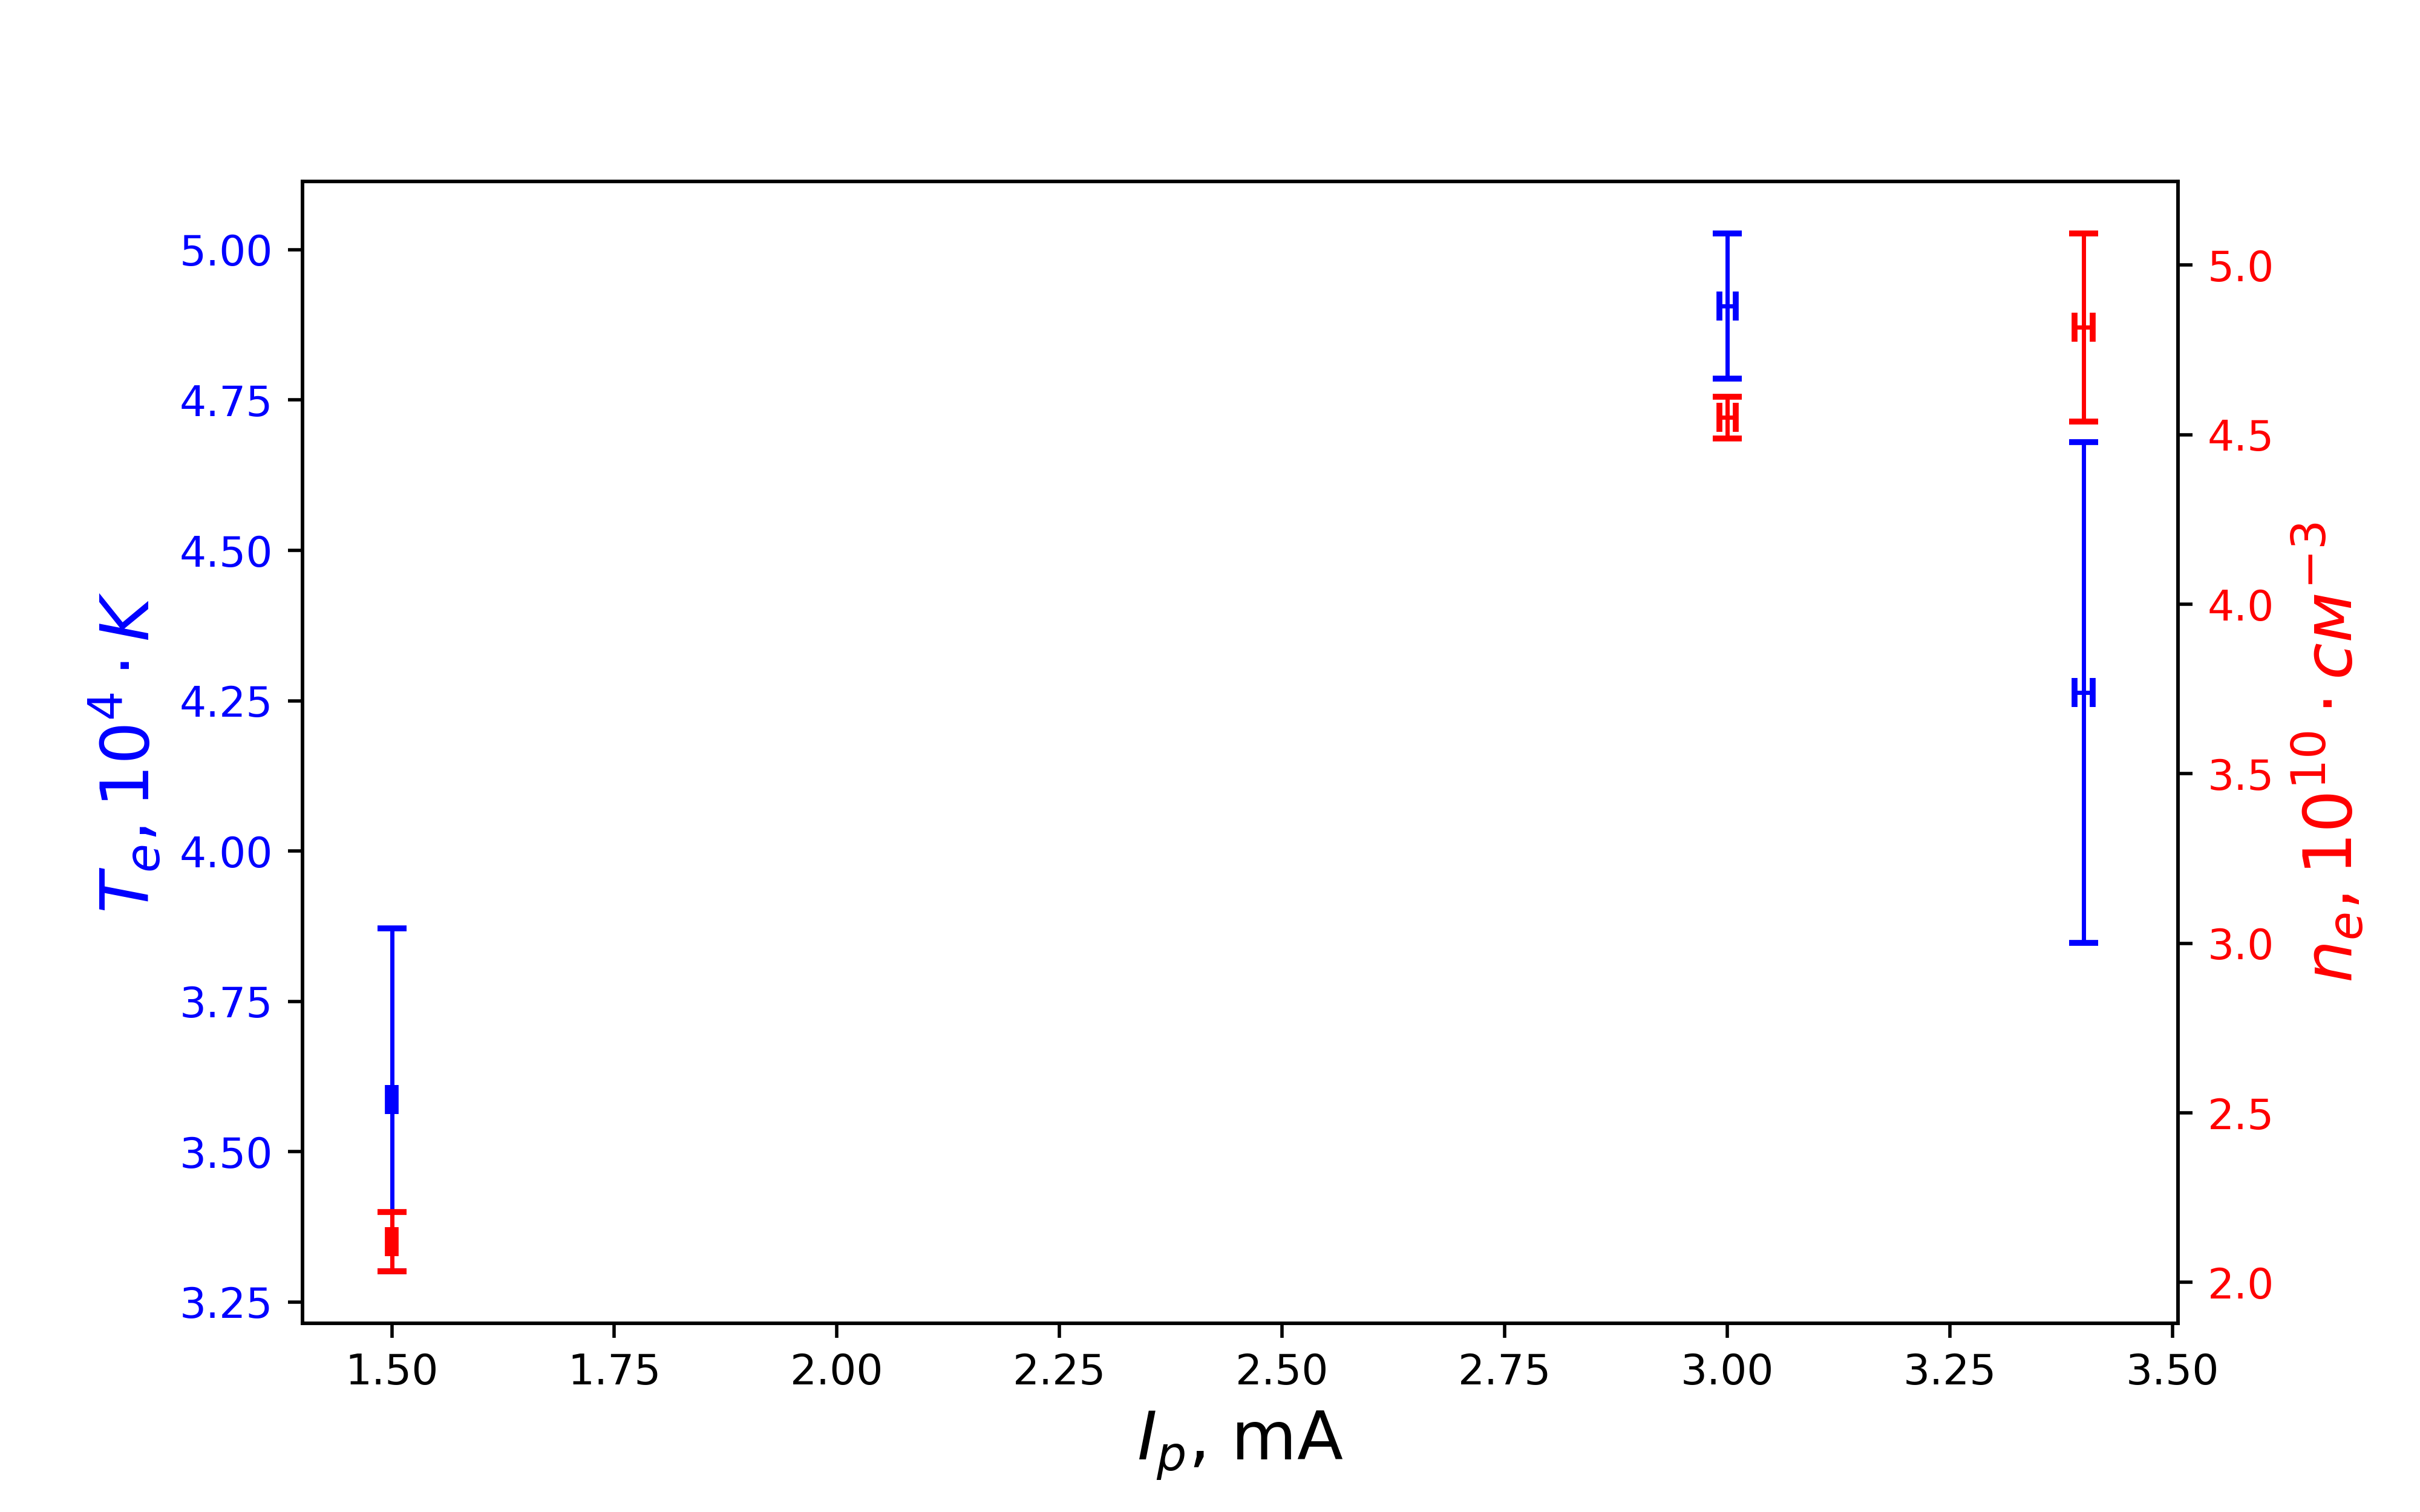
\includegraphics[width=\textwidth]{T,n(I_p)}
\caption{Зависимость электронной температуры и концентрации электронов от тока разряда} \label{от_тока_разряда}
\end{center}
\end{figure}

\section{Обсуждение результатов}


1.  При сравнении вольт-амперной характеристики разряда (рис. \ref{ВАХ_разряда}) и графика вольт-амперной характеристики газового разряда из приложения к лабораторной работе (рис. \ref{приложение}) видно, что рассматривался участок ГД, соответствующий поднормальному тлеющему разряду.

\begin{figure}[h!]
\begin{center}
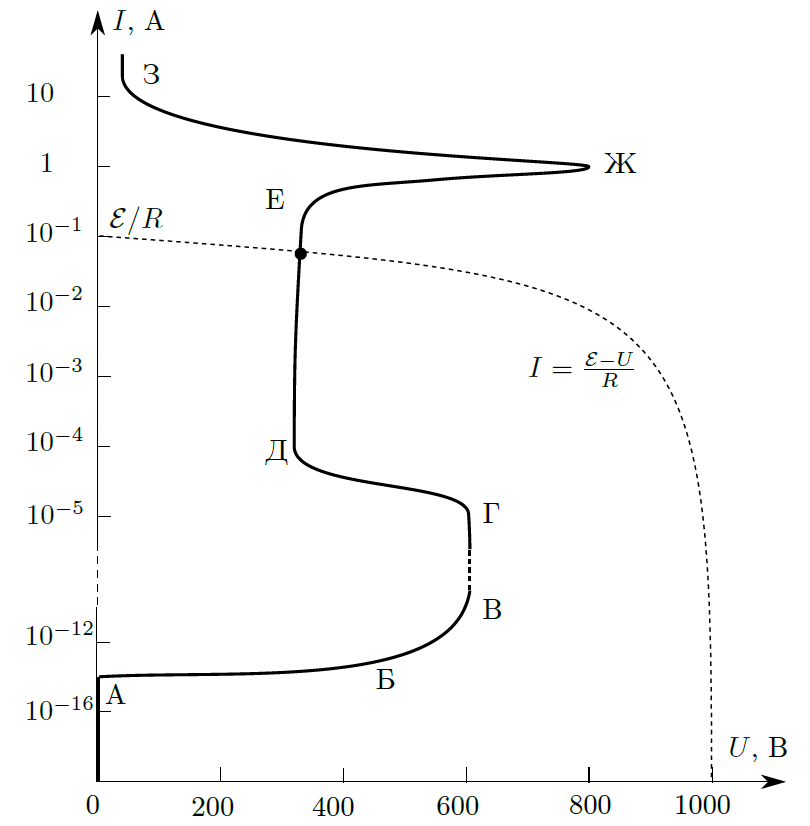
\includegraphics[width=0.5\textwidth]{Приложение}
\caption{Вольт-амперная характеристика разряда в неоне (из приложения)} \label{приложение}
\end{center}
\end{figure}

2. По определению поляризационной длины $r_{De}$ плазму можно считать квазинейтральной, так как именно электронная дебаевская длина определяет масштаб, на котором нарушается квазинейтральность из-за тепловых флуктуаций электронов относительно ионов, а $r_{De} \sim 10^{-2} см$, что много меньше размеров области.

3. Оценив число ионов в дебаевской сфере $N_D \sim 40$, видно, что число частиц много больше 1, что позволяет называть плазму идеальной.

4. Определить зависимость электронной температуры от тока разряда с помощью полученных данных (рис. \ref{от_тока_разряда}) невозможно из-за малого числа точек и достаточной погрешности результатов. Однако можно качественно оценить зависимость концентрации электронов от тока разряда: график напоминает линейную или степенную зависимость, что достаточно ожидаемо, при увеличении тока разряда увеличивается и число электронов в газе.


\section{Выводы}
Из ВАХ разряда подтверждено, что исследуется тлеющий газовый разряд. 
Экспериментальная зондовая характеристика подтверждает теоретическую зависимость: $I = I_{iн} th\frac{eU}{2k_БT_e}$, количество ионов в дебаевской сфере $N_D \sim 40$ показывает идеальность плазмы. Остальные характеристики плазмы получились схожими по порядку с примерами в инструкции к работе, что подтверждает справедливость метода измерений. Однако не удалось оценить зависимость температуры электронов от тока разряда из-за неточных измерений и малого их числа.

\end{document}